\documentclass[12pt]{article}
\usepackage{setspace}
\usepackage{graphicx} % used for includegraphics
\usepackage{url}
\singlespace
\usepackage[left=1in,right=1in,top=1in,bottom=1in]{geometry}


\title{\textbf{Comparing Vulnerabilitys in Networks: 
Software Defined and Software Managed Networks in Personal and Enterprise Networks}}
\author{Maxwell Stratford}

\begin{document}


\maketitle

\section{Introduction}
The world of computer networking and network security is a constantly changing field. Every day,
there is a new advancement, a new vulnerability, and a new attack. It can be hard to keep up with
this changing battlefield. My goal in this paper is to perform a penetration test on different
network formats and security protocols, and see how they differ in the way they detect and
resolve different network attacks. First, is to define the networks that I plan to test. 
I will start with personal home network type networks, with basic router settings to simulate 
the average home setup, and then try to secure the network using different network models, such 
as SDN (Software Defined Network), SMN (Software Managed Network), and, if I have extra time, AI 
Agentic networks. Then I will transfer into enterprise-sized networks, such as big businesses 
and college campus-type networks. At this time, I plan to use the software GHOSTs (created by 
Carnegie Mellon University)\cite{GHOSTSDocumentationGHOSTS} which runs on Docker, to simulate 
these types of networks, with realistic network traffic and setup. Through using this software, 
I will be able to simulate these networks for me to then penetration test them. I also plan on 
doing further research into the different types of attacks that I will be testing on these 
networks. So far, I have done research into the different types of people that are more 
susceptible to phishing attacks\cite{DemographicFactorsKavvadias}, and I plan on doing more
research into the different types of network attacks, such as DDoS, MITM, and more 
\cite{InternetFacingRouterRostami}. 
I will then be able to test these different types of attacks on the secured networks 
and see how they differ in their ability to detect and resolve these attacks. This will 
allow me to see how the different types of networks differ in their security and 
vulnerability, and how they can be improved to better protect against these types of attacks,
and see how some Network Technicians, would have to make the best decision on which type of 
network to use for their specific needs, and how they can best secure their network against 
these types of attacks. A basic enterprise network, which will be among the first networks tested, 
might look something like this. With a router at the top, sending packets(data) to different switches
which would in turn, send data to the end user computers. I will implement basic network security
such as no open ports on the router and switches, Spanning tree protocol on the switches, and 
Ingress filtering. A basic home network usually would just consist on a router(at the top) connected
directly to the end users devices through ethernet or wifi.\cite{thewifiofthings} \ref{fig:network}.

\begin{figure}[h]
\begin{center}
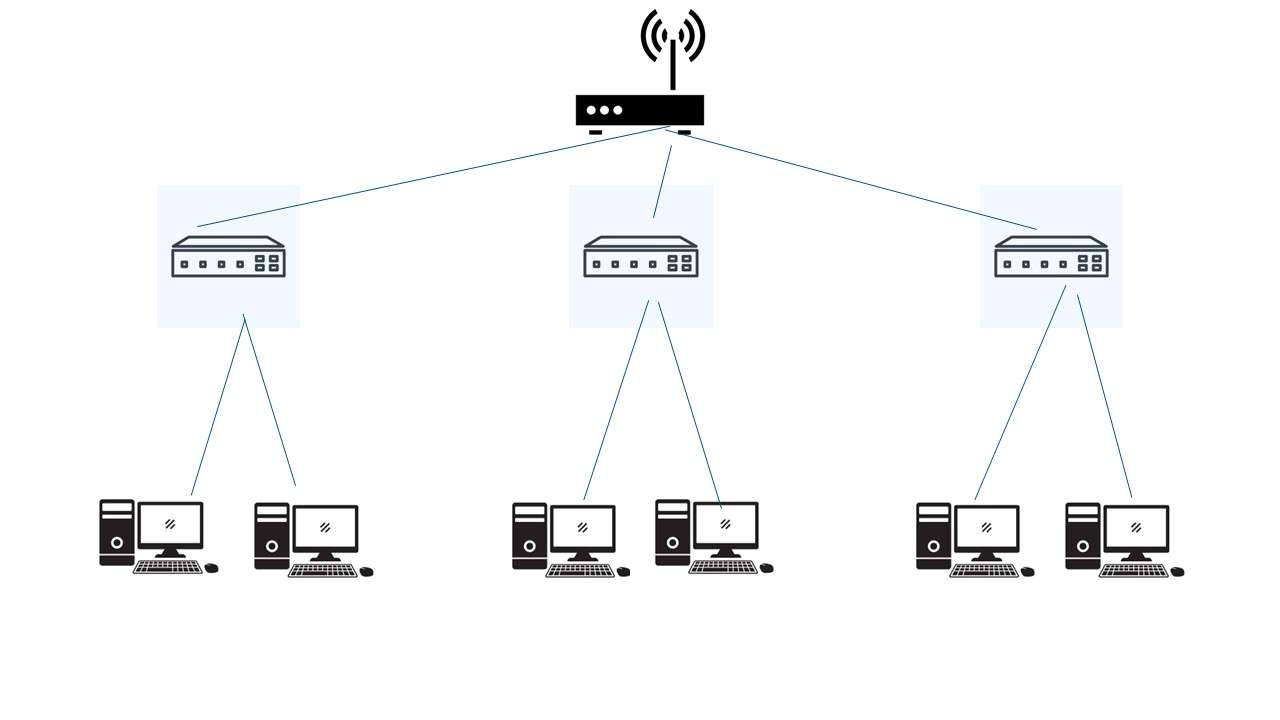
\includegraphics[scale=0.4]{BasicNetwork.jpg}
\caption{A basic enterprise type network consisting of a router, three switches, and six end user computers.
and a ethernet connection between the router and switches, and between the switches and end user computers.}
\label{fig:network}
\end{center}
\end{figure}


\newpage
\section*{Appendix}
A list of planned test so far, which may be added to as I do more research into the different types of 
attacks and networks. Attack types will include, but are not limited to, DDoS, MITM and Phishing. 
A Strech goal of mine is to also test on AI Agentic Networks, which is a new type of network that 
uses AI to detect and resolve network attacks. 
\begin{itemize}
	\item Test 1: Attacks on Personal Home Network with Basic Router Settings
	\item Test 2: Attacks on Personal Home Network with SDN
	\item Test 3: Attacks on Personal Home Network with SMN
	\item Test 4: Attacks on Enterprise Network with Basic Router Settings
	\item Test 5: Attacks on Enterprise Network with SDN
	\item Test 6: Attacks on Enterprise Network with SMN
	\item Test 7: Attacks on Enterprise Network with AI Agentic Network
\end{itemize}


\bibliographystyle{acm}
\bibliography{bibliography.bib}

\end{document}
